\documentclass{scrartcl}

\usepackage[hidelinks]{hyperref}
\usepackage[none]{hyphenat}
\usepackage{graphicx}
\graphicspath{{images/}}

\title{Portfolio Proposal}
\subtitle{COMP220}

\author{Warwick New(15002903)}

\begin{document}

\maketitle

\section*{Concept}
In this demo I plan to make  a relaxing walking simulater which draws inspiration from games like Proteus \cite{proteus} and Drizzle Path \cite{drizzlepath}, mainly focusing on points from the former of the two ``games''.

\begin{figure}[h]
	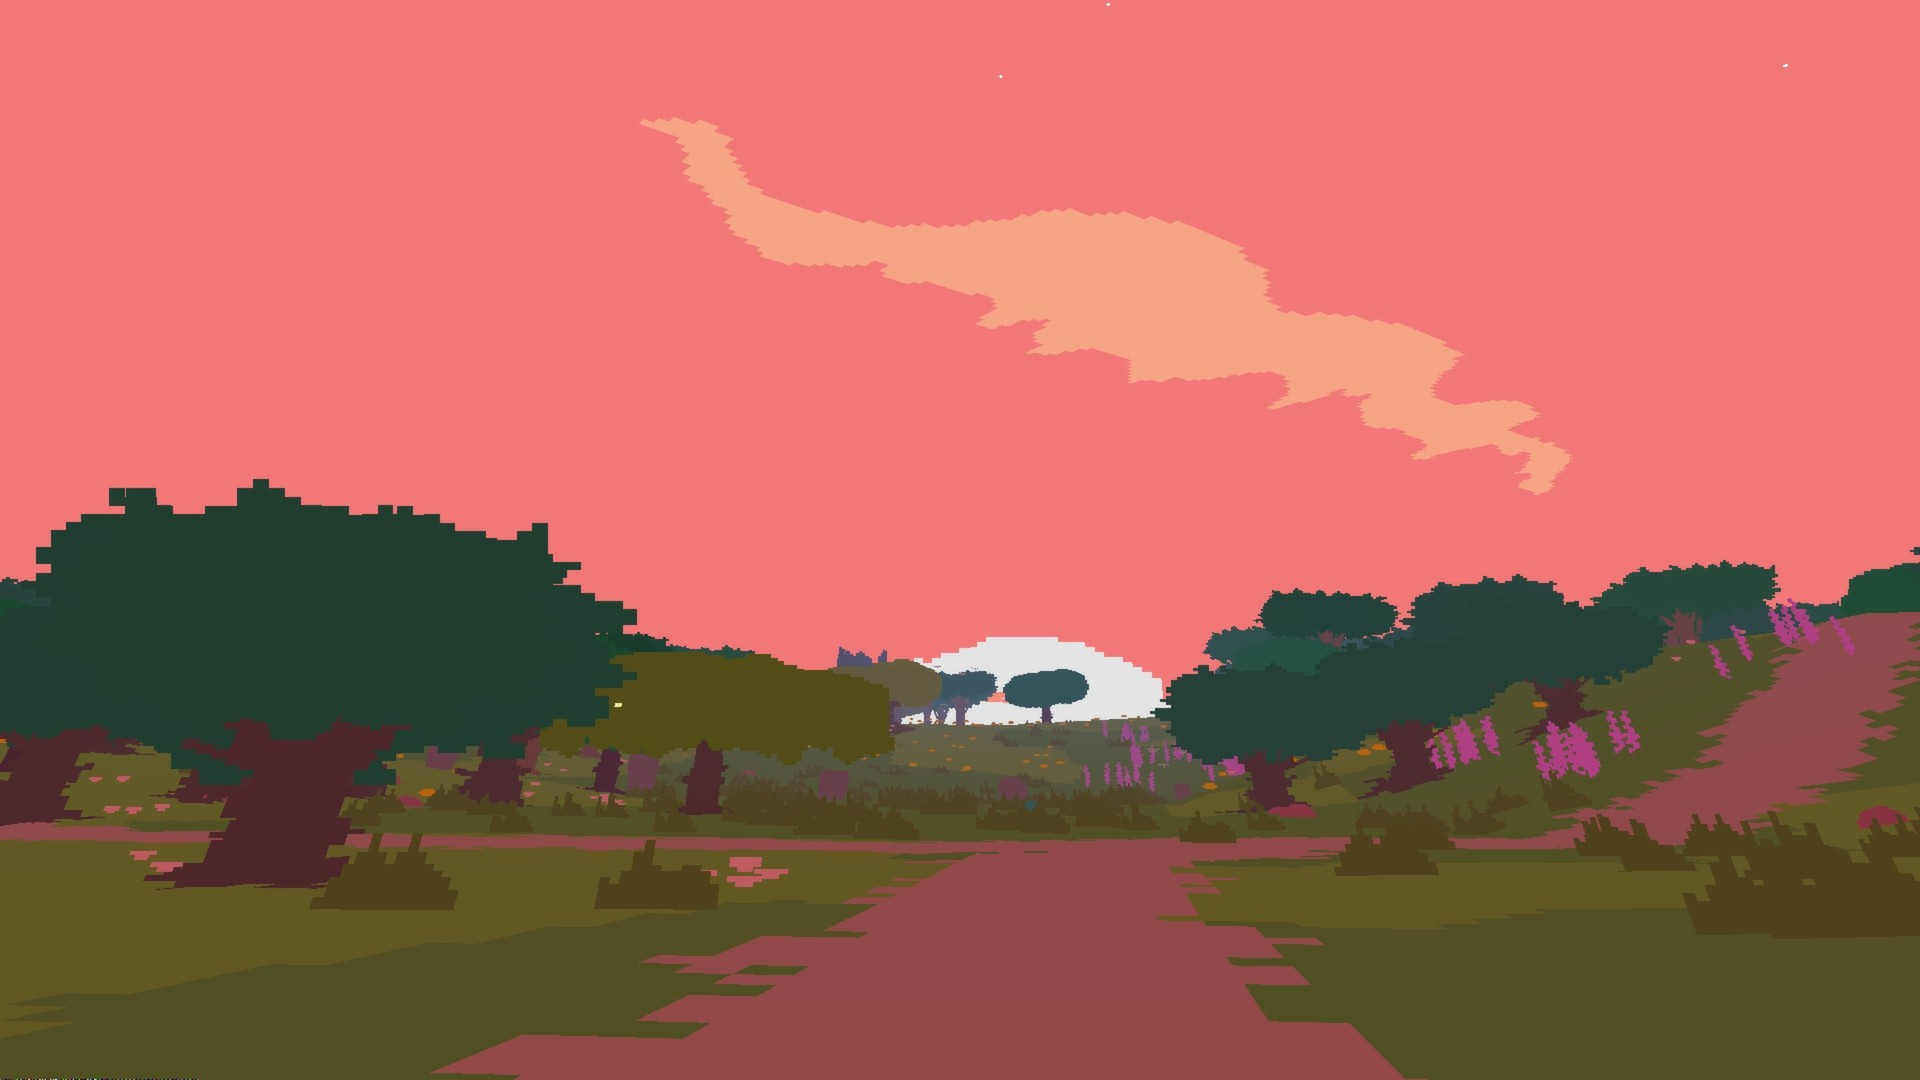
\includegraphics[width=8cm]{Proteus}
	\centering
\end{figure}

\begin{figure}[h]
	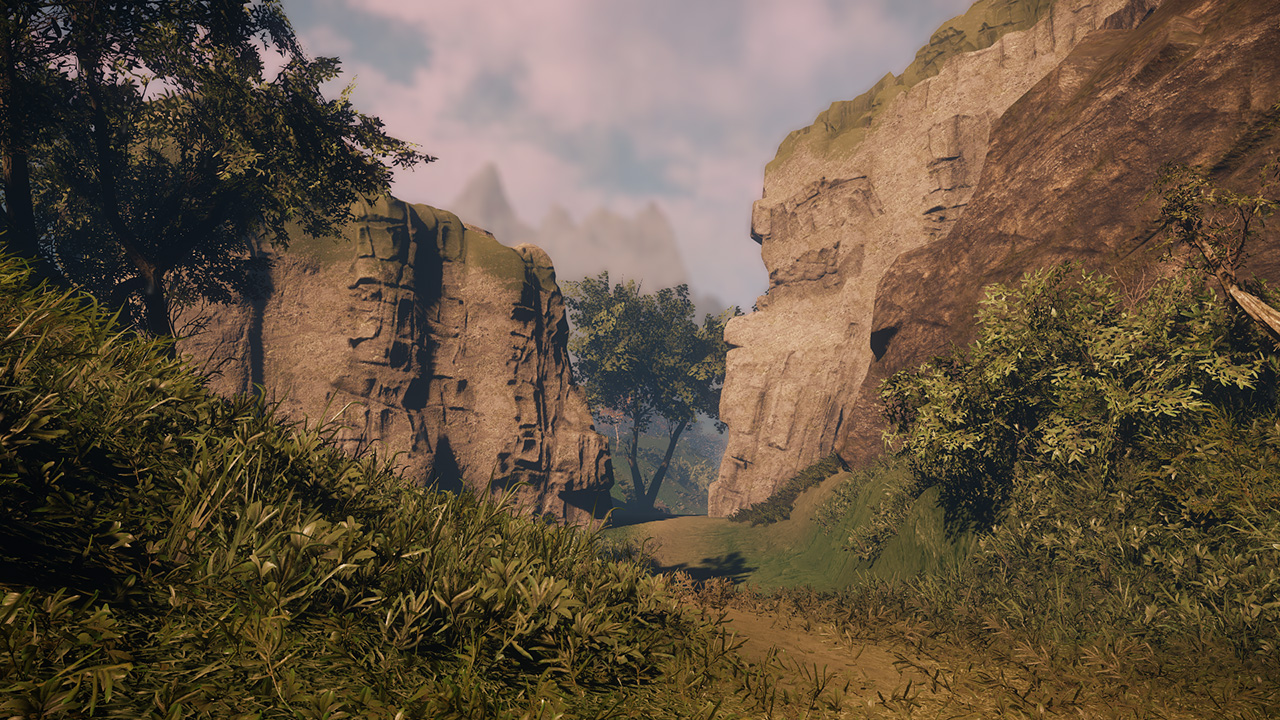
\includegraphics[width=8cm]{DrizzlePath}
	\centering
\end{figure}

In order to achieve this effect I plan on making a simple random terrain generation algorithm and as a stretch goal potentially populating the terrain with other objects. I chose to add a PCG aspect to allow for replay ability in the project and to push the responsibility of any kind of narrative away from me. In order to achieve the intended aesthetic I will attempt to use a single set of colours that will match those potentially with a sunset sky and will also attempt to add shadows to give the terrain (Of which will more than likely be pretty bare) some definition. However with a world to walk around in The project will likely require some kind of collision detection, to allow the user to walk freely without clipping through the terrain. However I wish this demo to be focused on the aesthetic first and the functionality of the players movement second. Given that the level is procedurally generated, another potential stretch goal is to dynamically generate more terrain as you travel however I will not likely have enough time to implement this.

\section*{Describe}
\subsection*{Terrain}
I will attempt to generate terrain using a height map stored in a 2 dimensional form of vector, where I will select several random points and give them random heights within a reasonable range. I will then attempt to smooth the points in between these raised or lowered points to make hills or valleys.
\subsection*{Shadows}
I will also attempt to generate a shadow map with the level to give each generation of terrain its own matching shadows and will then attempt to render it on the screen I will also attempt to solve any shadow acne issues that arise by adding a error margin where necessary.

\appendix
\section{Goals}
\subsection{Procedural generation of complex meshes or terrain}
\subsection{An advanced real-time lighting effect (e.g. shadow casting)}
\section{Stretch Goals}
\subsection{Collision detection or ray-casting}
\bibliographystyle{ieeetr}
\bibliography{HandOut}

\end{document}